\documentclass[crop,tikz]{standalone}
\usetikzlibrary{positioning,arrows,fit,calc}
\pgfdeclarelayer{bg}
\pgfsetlayers{bg,main}
\tikzset{
	>=stealth'
}
\begin{document}
	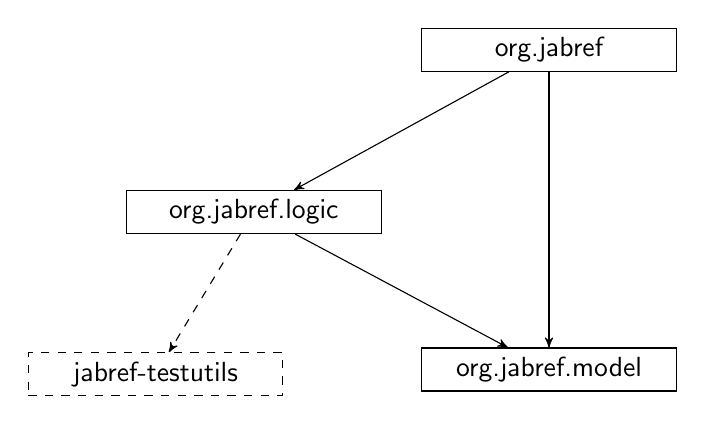
\begin{tikzpicture}[
	node distance = 2mm,
	every node/.style = {
		font = \sffamily
	},
	module/.style = {
		draw,
		text width = 3cm,
		align = center,
	}
	]
	
	\node[module] (jabref) {org.jabref};
	\node[module, below = 35mm of jabref] (model) {org.jabref.model};
	\node[module, below left = 15mm and 5mm of jabref] (logic) {org.jabref.logic};
	\node[module, below left = 15mm and -20mm of logic, dashed] (test) {jabref-testutils};
	
	\draw[->] (jabref) -- (logic);
	\draw[->] (jabref) -- (model);
	\draw[->] (logic) -- (model);
	\draw[->, dashed] (logic) -- (test);
		
	\end{tikzpicture}
	
\end{document}